\documentclass[11pt,a4paper]{article}
\usepackage{helvet} 
\renewcommand{\familydefault}{\sfdefault}
\usepackage{a4wide}
\usepackage{ucs}
\usepackage[utf8x]{inputenc}
%\usepackage[english]{babel}
\usepackage[portuges]{babel}
\usepackage{graphicx}
\usepackage{cite}
\usepackage[absolute]{textpos}
\usepackage{fancyhdr}
\usepackage{amsfonts}
\usepackage[table]{xcolor}
\usepackage{UnBTitle}
\usepackage{etoolbox}
\usepackage{listings}
\usepackage{float}% Para o uso da opção [H] de flutuação das imagens

\renewcommand{\lstlistingname}{Código}

% Configuracao de lstlistings
\lstdefinestyle{customc}{
  belowcaptionskip=1\baselineskip,
  breaklines=true,
  frame=L,
  xleftmargin=\parindent,
  language=C,
  showstringspaces=false,
  basicstyle=\footnotesize\ttfamily,
  keywordstyle=\bfseries\color{green!40!black},
  commentstyle=\itshape\color{purple!40!black},
  identifierstyle=\color{blue},
  stringstyle=\color{orange},
}

\departamento{
Fundamentos Computacionais de Robótica \\
Departamento de Ciência da Computação - CIC - UnB \\
Prof. Carla Cavalcante Koike
}

\title{
Trabalho 2 - Abordagem para Desvio de Obstáculos utilizando Robô Pioneer 3AT
}

\author{
Andressa Sousa da Silveira - 10/0053971 \\
Lucília Pereira de Oliveira - 12/0045397 \\
Matheus Medeiros Sarmento - 12/0053161 \\
Rondinele Barbosa Prado - 10/0039880 \\
%
}
\begin{document}
\maketitle
\lstset{language=C++} 


\thispagestyle{empty}
\pagestyle{empty}
%%%%%%%%%%%%%%%%%%%%%%%%%%%%%%%%%%%%%%%%%%%%%%%%%%%%%%%%%%%%%%%%%%%%%%%%%%%%%%%%%%%

\section{Introdução}
Os robôs estão cada vez mais autônomos, e quando se trata de
exploração de um ambiente, uma importante tarefa que ele deve estar
apto a realizar é a prevenção de obstáculos em seu caminho. Essa
tarefa é dinâmica, ou seja, não é necessário ter um conhecimento
prévio do ambiente em que o robô se encontra, contando apenas com
algoritmos que trabalham com dados recebidos pelos
sensores. Tipicamente, o desvio de obstáculos recebe instruções de
outro módulo (geralmente o planejador de rota) que indica qual direção
ele deve seguir, e assim, decide o movimento que o motor deve realizar
baseado nos dados que os sensores fornecem, realizando, portanto, uma
interface entre o módulo de decisão de caminho e o motor do robô.
Atualmente, existem diversos algoritmos que propõem a resolução do
desvio de obstáculos. O utilizado neste projeto foi o Vector Field
Histogram(VFH).

\section{Metodologia}
Para a implementação do código que controla o robô, foram
utilizados dois métodos: o (1) \textit{Vector Field Histogram} (VFH)
\cite{c1}; e a técnica de (2) \textit{Bubble Band} \cite{c3}.
\\

\subsection{VFH}
\label{sec:vfh}

O VFH é um método desenvolvido para robôs-móveis evitarem obstáculos em tempo real, permitindo a
detecção de obstáculos desconhecidos ao mesmo tempo em que o robô se desvia destes em direção
ao objetivo. Em uma primeira etapa, o método utiliza uma grade de histograma cartesiano bidimensional $C$ para a representação dos obstáculos, que é frequentemente atualizada a cada taxa de dados amostrados pelos sensores do robô enquanto ele se move. Cada célula $(i,j)$ na grade de histograma contém um valor $c_{i,j}$, que representa a probabilidade de existir um obstáculo naquele local. A cada leitura de amostras, apenas uma célula a uma distância $d$ do sensor terá seu valor incrementado, resultando em um histograma de distribuição de probabilidade, no qual valores de alta certeza estarão em células próximas à atual posição de um obstáculo. A Figura \ref{fig:histog_dist_prob} mostra o quanto esta tática faz com que a mesma célula e as suas vizinhas sejam repetidamente incrementadas.

\begin{figure}[H]
    \centering
    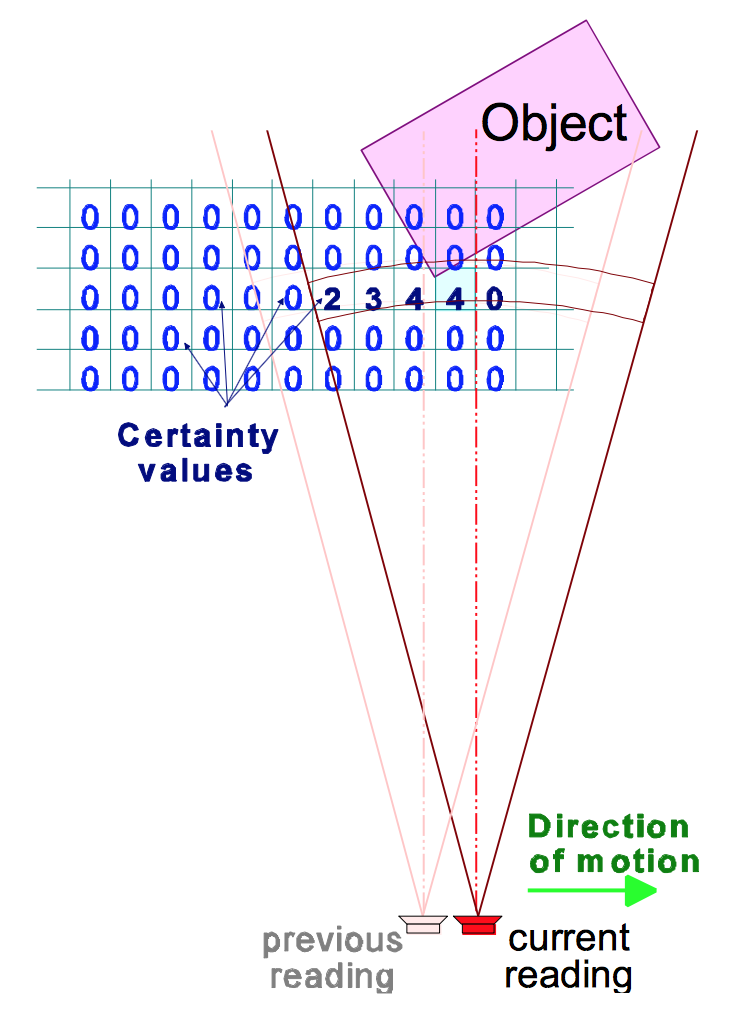
\includegraphics[width=0.4\textwidth]{img/histog_dist_prob}
    \caption{Histograma de distribuição de probabilidade. Fonte: \cite{c1}}
    \label{fig:histog_dist_prob}
\end{figure}

Em seguida, em uma etapa intermediária, a grade de histograma $C$ é reduzida em um histograma polar unidimensional $H$, que é construído de acordo com a localização momentânea do robô. $H$ consiste em $n$ setores de largura $\alpha$, cujo conteúdo é um valor que representa a densidade do obstáculo polar naquela direção. O mapeamento de $C$ em $H$ (Figura \ref{fig:map_grid_polar}) é realizado da seguinte forma: existe em $C$ uma janela de $w_{s} \times w_{s}$ células que se move junto do robô, chamada de região ativa $C^{*}$. As células ativas serão tratadas como um vetor de obstáculo, cuja direção $\beta$ será a medida da direção da célula até o centro do veículo. Desse modo, a direção $\beta$ é determinada por

\begin{figure}[H]
    \centering
    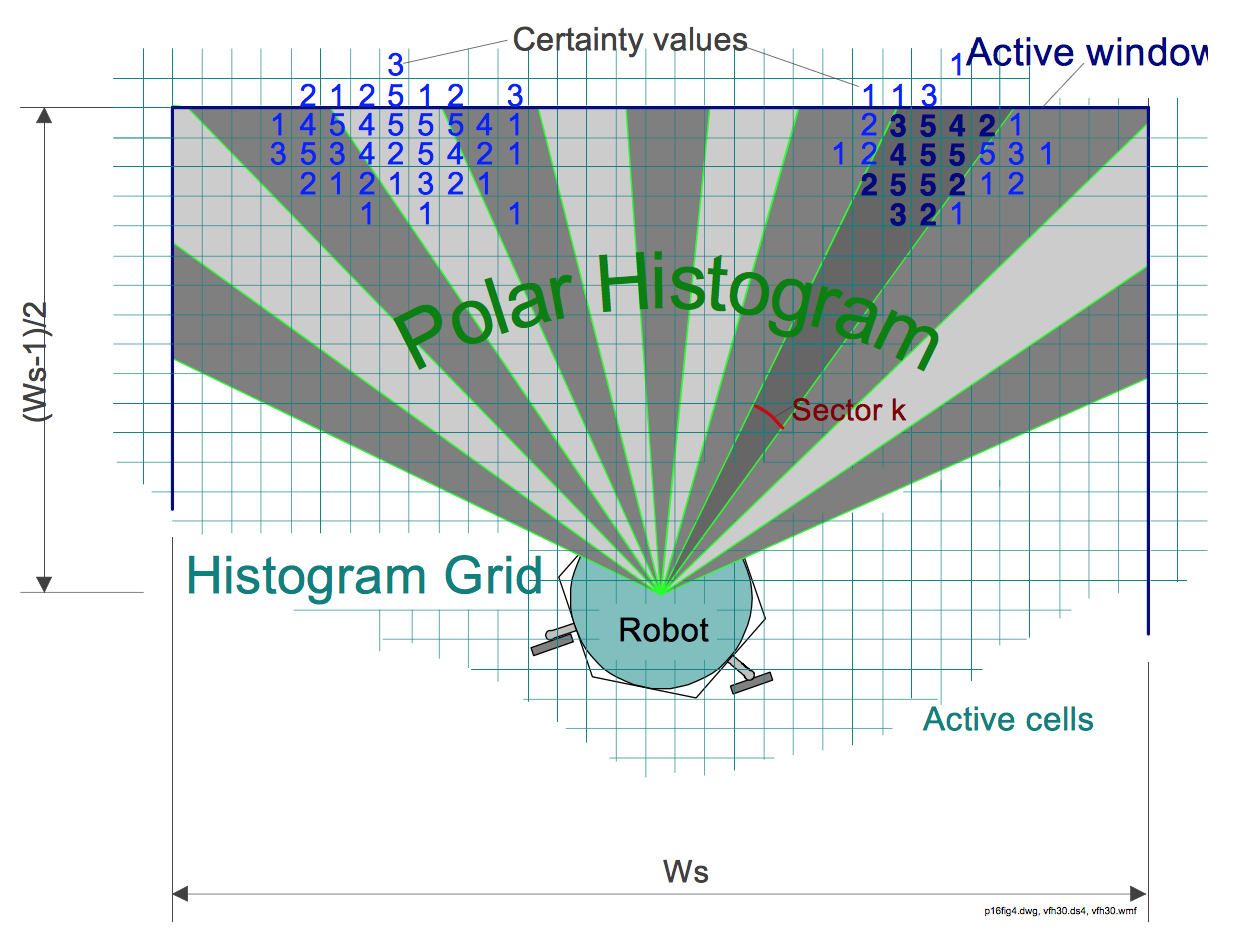
\includegraphics[width=0.8\textwidth]{img/map_grid_polar}
    \caption{Mapeamento das células ativas para o histograma polar $H$. Fonte: \cite{c1}}
    \label{fig:map_grid_polar}
\end{figure}

$$\beta = \tan^{-1}\frac{y_{i}-y_{0}}{x_{i}-x_{0}}$$

onde $x_{0}$ e $y_{0}$ são as coordenadas do centro do robô e $x_{i}$ e $y_{i}$ são as coordenadas da célula ativa $(i,j)$.
\\

A magnitute do vetor de obstáculo será dada por

$$m_{i,j} = (c^{*}_{i,j})^{2} (a - bd_{i,j})$$

onde $c^{*}_{i,j}$ é o valor de certeza da célula ativa $(i,j)$, $d_{i,j}$ é a distância entre a célula ativa $(i,j)$ e o centro do robô e $a$,$b$ são constantes positivas.
\\

A correspondência entre $c^{*}_{i,j}$ e o setor $k$ de $H$ é determinada através de

$$k = INT(\frac{\beta_{i,j}}{\alpha})$$

Para cada setor $k$, a densidade do obstáculo polar $h_{k}$ é calculada por

$$h_{k} = \sum_{i,j} m_{i,j}$$
\\

O resultado desse mapeamento pode gerar erros devido à natureza discreta da grade de histograma, por isso uma função de suavização é aplicada em $H$, obtendo a densidade de obstáculo polar suavizada $h'_{k}$ (POD).
\\

Nas Figuras \ref{fig:config_obs_grid_histog} e \ref{fig:polar_histog} é mostrado um exemplo de como essas duas etapas, a inicial e intermediária, são construídas.

\begin{figure}[H]
\centering
\begin{minipage}{.5\textwidth}
  \centering
  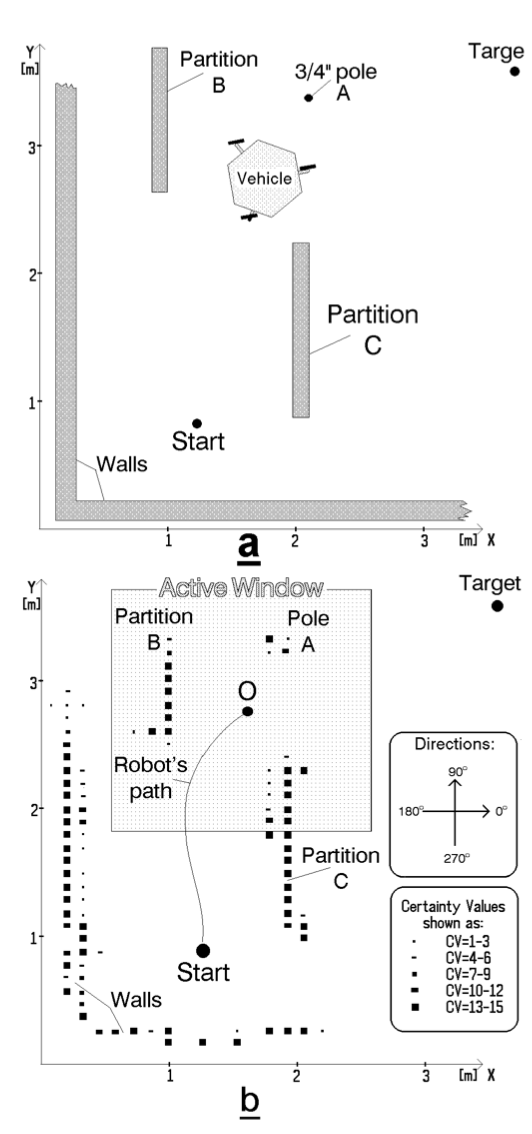
\includegraphics[width=.8\linewidth]{img/config_obs_grid_histog}
  \captionof{figure}{\textbf{a.} Exemplo de uma configuração de obstáculos. \textbf{b.} A representação da grade de histograma correspondente a o que está em \textit{a}. Fonte: \cite{c1}}
  \label{fig:config_obs_grid_histog}
\end{minipage}%
\begin{minipage}{.5\textwidth}
  \centering
  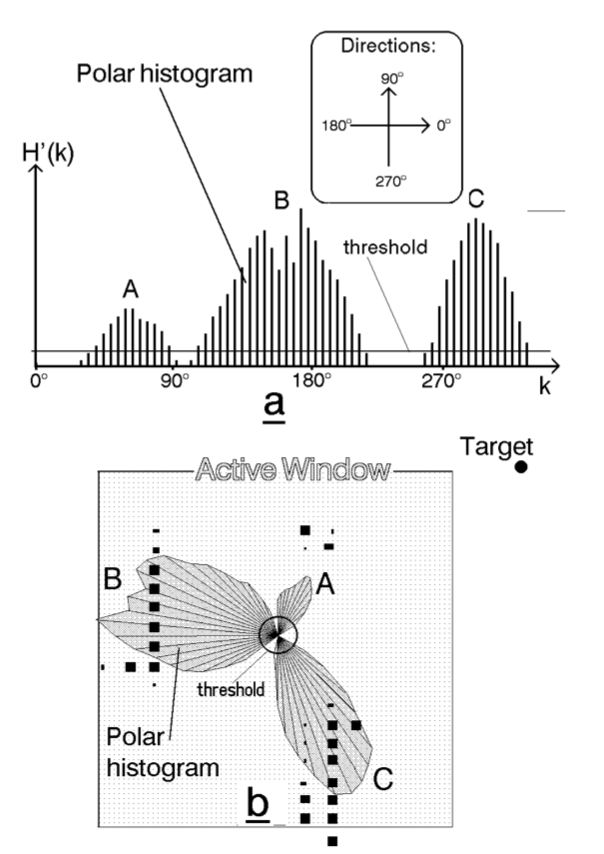
\includegraphics[width=.8\linewidth]{img/polar_histog}
  \captionof{figure}{\textbf{a.} A representação da densidade do obstáculo polar no histograma polar $H$ relativa à posição do robô em $O$. \textbf{b.} O histograma polar mostrado em \textit{a} na forma polar sobreposto pela grade de histograma mostrada na Figura \ref{fig:config_obs_grid_histog}b Fonte: \cite{c1}}
  \label{fig:polar_histog}
\end{minipage}
\end{figure}

%\begin{figure}[H]
%    \centering
%    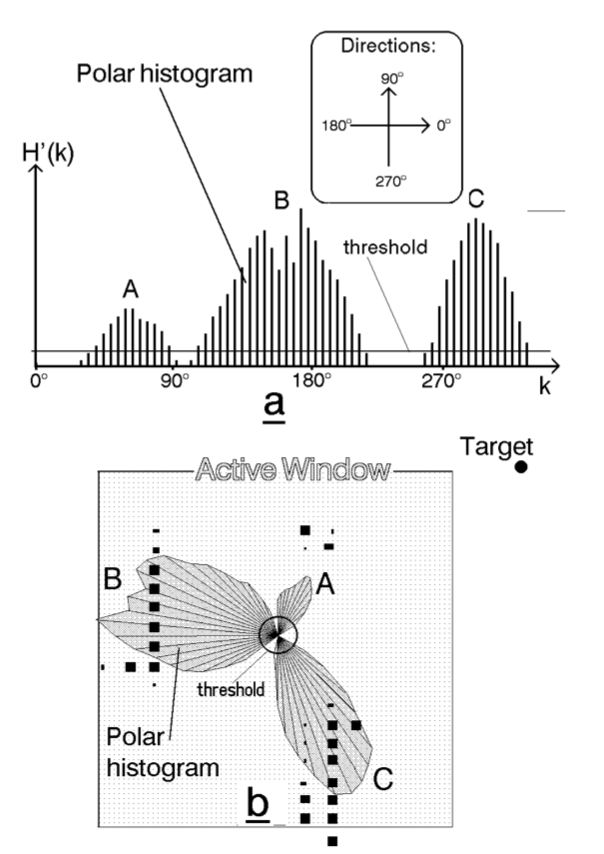
\includegraphics[width=0.55\textwidth]{img/polar_histog}
%    \caption{Histograma polar de magnitudes, com um valor empírico de limiar(threshold) de definição de um vale. Fonte: \cite{c1}}
%    \label{fig:polar_histog}
%\end{figure}

Na última etapa do método VFH, é computada a saída do algoritmo, que é a direção $\theta$ necessária para o robô girar se desviando do obstáculo.
\\

Um histograma polar possui "picos", setores com altos PODs,  e "vales", setores com baixos PODs. Qualquer \textit{vale} pertencente a um certo limiar é chamado de \textit{vale candidato}. Geralmente, há dois ou mais \textit{vales candidatos} e o algoritmo escolhe aquele que mais corresponde com a direção do objetivo $k_{targ}$.	 Uma vez que um \textit{vale} é escolhido, é necessário encontrar um setor apropriado do \textit{vale}.

O algoritmo mede a quantidade de setores no \textit{vale} para determinar se ele é um \textit{vale} \textit{largo} ou \textit{estreito}. Um \textit{vale largo} ocorre quando seu número de setores consecutivos dentro do limiar ultrapassou o valor $s_{max}$. O setor mais próximo de $k_{targ}$ é denotado por $k_{n}$ e $k_{f}$ é definido por $k_{f} = k_{n}+s_{max}$, ficando mais longe da borda. A direção de giro $\theta$ desejada é calculada por $\theta = \frac{(k_{n} + k_{f})}{2}$. Na Figura \ref{fig:cand_direc} é mostrado um exemplo de quais direções podem ser escolhidas para que um robô contorne os obstáculos. 

\begin{figure}[H]
    \centering
    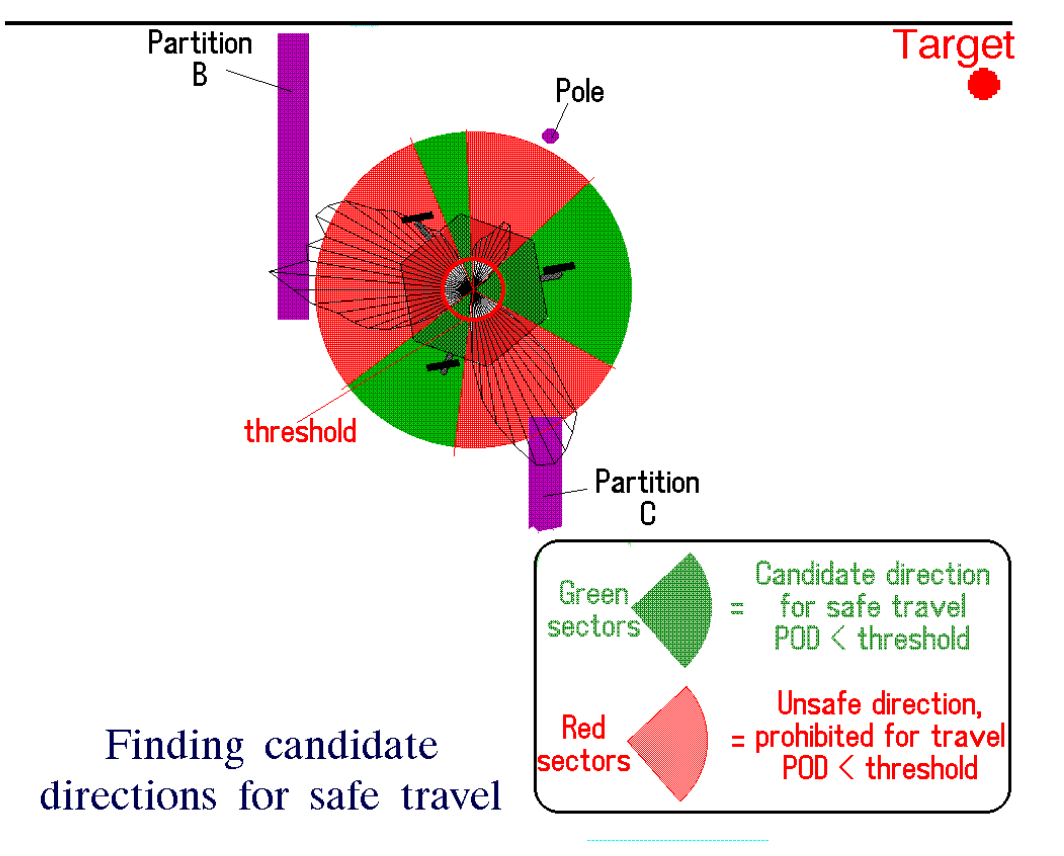
\includegraphics[width=0.6\textwidth]{img/candidate_directions}
    \caption{O limiar de um histograma polar determina as direções candidatas para um viagem segura. Fonte: \cite{c1}}
    \label{fig:cand_direc}
\end{figure}

\subsection{Técnica de Bubble Band}
\label{sec:bubbleband}

A técnica de \textit{Bubble Band} consiste em um método que define uma "bolha", a qual representa a distância livre necessária ao entorno do robô para que ele se desloque sem que haja colisão. A forma da bolha pode variar de acordo com a estrutura do robô, de modo que esta se encaixe na geometria do mesmo.

\begin{figure}[H]
    \centering
    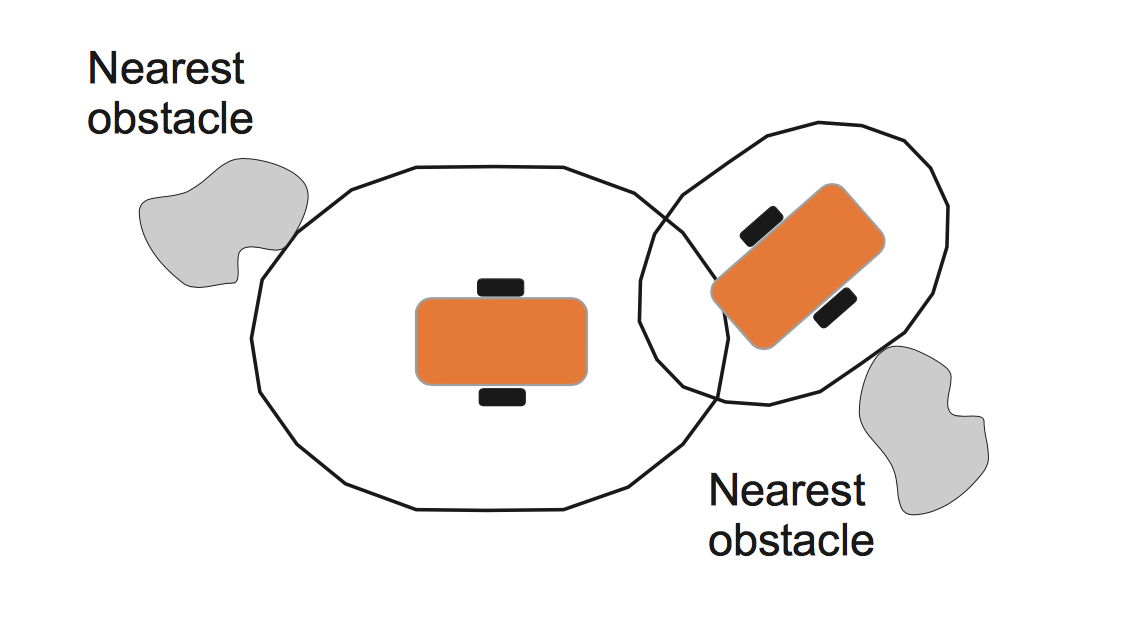
\includegraphics[width=0.6\textwidth]{img/bubble}
    \caption{Técnica de Bubble Band. Fonte: \cite{c2}}
    \label{fig:bubble}
\end{figure}


\section{Condições de Funcionamento}
Para o correto funcionamento da atual implementação, assume-se que o Pioneer 
será equipado com um sensor laser.

As condições do ambiente devem ser um terreno plano e com espaço suficiente para que o Pioneer possa se 
deslocar. Além disso, o terreno não deve ser escorregadio, para evitar colisões inesperadas. 
 
Os obstáculos não podem se movimentar com uma velocidade elevada quando próximos ao robô, pois, caso contrário, o robô poderá não ter tempo suficiente para calcular a nova rota, causando uma colisão com o obstáculo. 
Por fim, os obstáculos devem possuir textura e coloração refletora e altura mínima, de forma que o laser consiga detectá-los.

O algoritmo VFH planeja o caminho apenas localmente e, dessa forma, 
não tenta achar um caminho otimizado para o robô, implicando que este pode 
ficar “preso” indefinidamente em algumas situações. Neste caso, ele geralmente andará em círculos ou 
circulará em torno de um conjunto de obstáculos próximos.


\section{Algoritmos Implementados}
O algoritmo responsável por efetuar o desvio de obstáculos recebe como
entrada um vetor indicando a direção e a velocidade a serem aplicadas
ao robô e as leituras do laser. Ele retorna um novo vetor
representando a direção e velocidade calculadas de modo que o robô
tenda a seguir na direção desejada, desviando de eventuais obstáculos.
O vetor de direção é representado por uma mensagem do tipo
\lcode{geometry\_msgs/Twist}. As leituras do laser são representadas
por mensagens do tipo \lcode{sensor\_msgs/LaserScan}. Um diagrama
contendo os nós e tópicos utilizados pelo sistema podem pode ser
observado na Figura \ref{fig:diag_proj_ros}.

\begin{figure}[H]
    \centering
    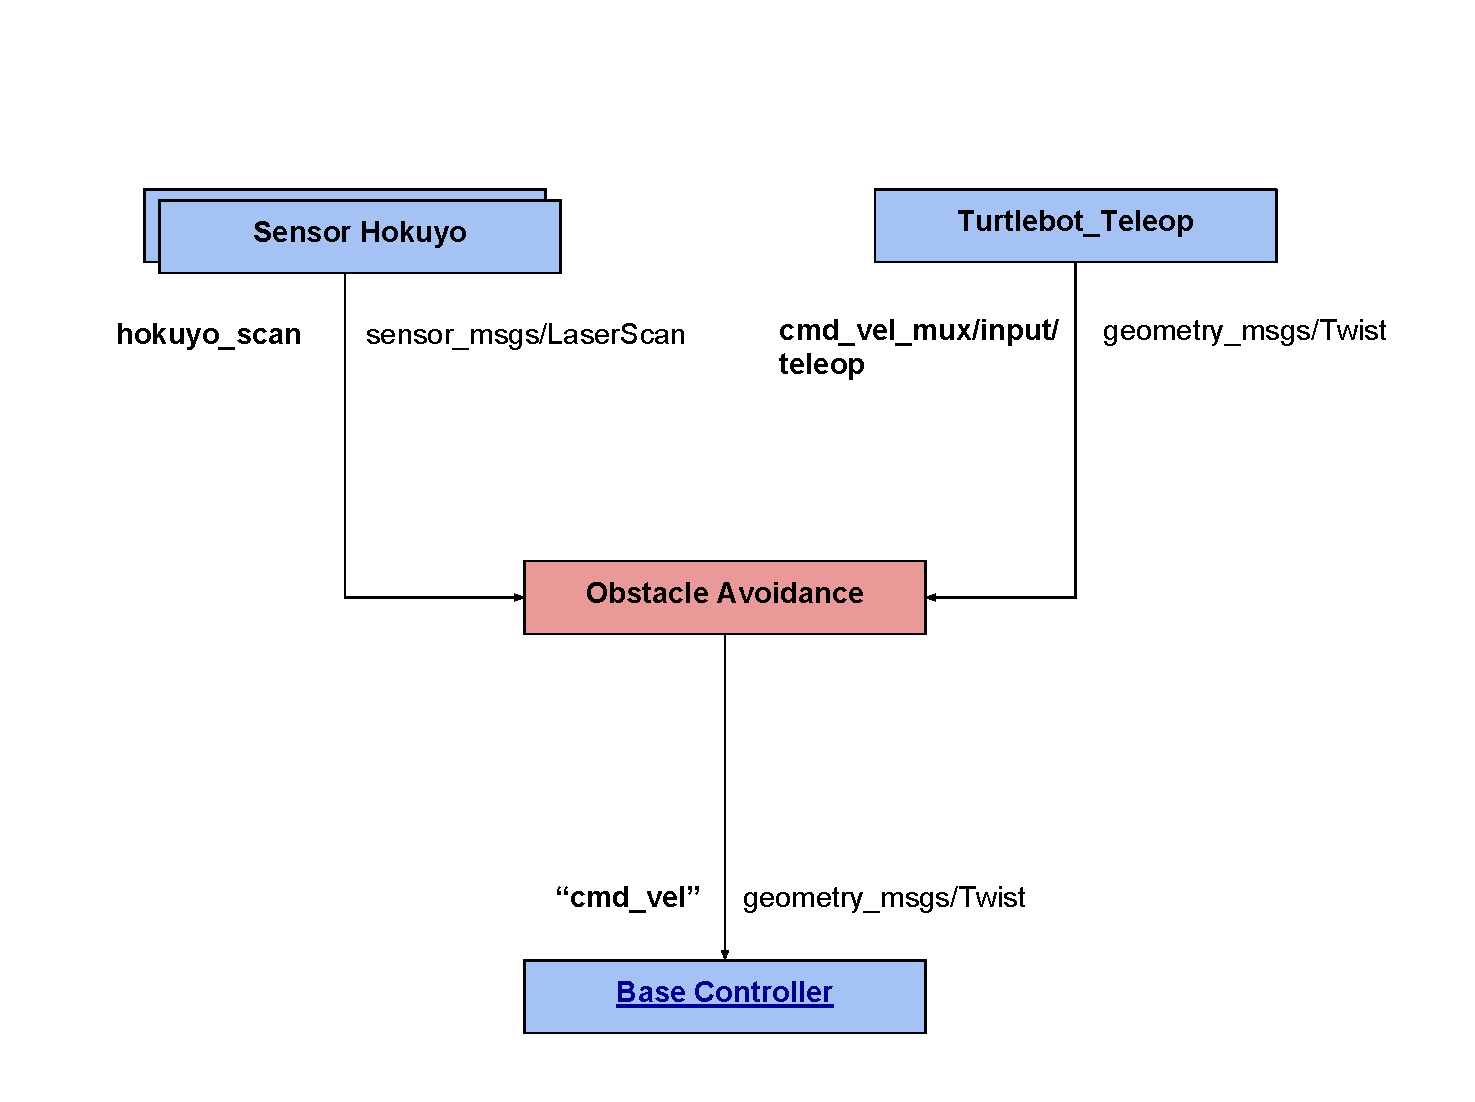
\includegraphics[width=0.85\textwidth]{img/Diagrama_Projeto_ROS.pdf}
    \caption{Diagrama de nós do sistema}
    \label{fig:diag_proj_ros}
\end{figure}

O tópico \lcode{hokuyo\_scan} fornece as leituras do laser, e o tópico
\lcode{cmd\_vel\_mux/input/} fornece os vetores indicando a direção que
o robô deve seguir. O módulo \textbf{Obstacle Avoidance} representa o
algoritmo de desvio de obstáculos, o qual posta os vetores resultantes
no tópico \lcode{cmd\_vel} do robô.

\subsection{Detecção de Obstáculos}

Foi utilizado um algoritmo do tipo ``bolha'', o qual detecta a
presença de obstáculos que ultrapassem uma determinada distância
limite (envoltório da bolha). Esta distância limite visa assegurar que
o robô evite colisões. Caso alguma amostra do sensor aponte um valor
de distância menor que o limite, é chamado o algoritmo VFH. Como o
laser utilizado fornece aproximadamente 728 amostras de distâncias
(\textit{ranges}), 40 vezes por segundo, decidiu-se verificar a cada
dez amostras a presença de obstáculos, de $-90°$ a $+90°$ em relação
ao eixo central do robô (Figura \ref{fig:laser_scan}). O algoritmo de
detecção de obstáculos implementado pode ser observado no Código
\ref{cod:checkObstacles}.

\begin{figure}[H]
    \centering
    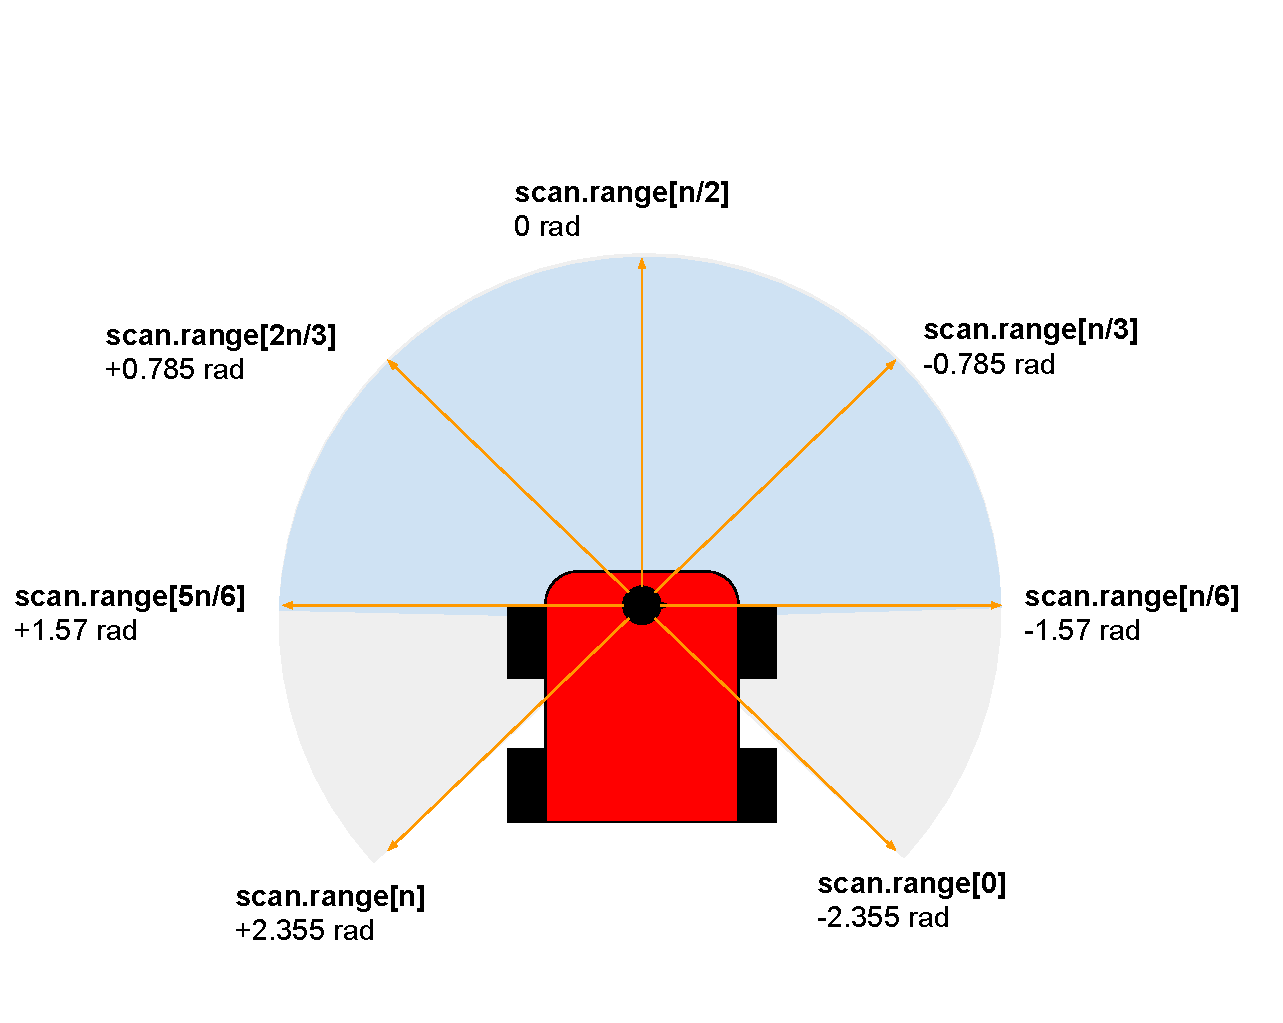
\includegraphics[width=0.85\textwidth]{img/SensorAngulos.pdf}
    \caption{Leitura do sensor laser}
    \label{fig:laser_scan}
\end{figure}

\begin{lstlisting}[frame=single, label=cod:checkObstacles, style=customc,
caption={Algoritmo de Verificação de Obstáculos}]
bool checkForObstacles(sensor_msgs::LaserScan msg, float limite){
    
    int numero_amostras = (int) floor((msg.angle_max - msg.angle_min) / msg.angle_increment);
    
    //Le as amostras a cada 10 unidades
    for (int i = 0; i < numero_amostras; i+= 10){
        if(i > numero_amostras/6 && i < 5*numero_amostras/6) //90 graus
            if (msg.ranges[i] < limite) return true;
    }
    return false;
}
\end{lstlisting}


\subsection{VFH}

Primeiramente, o VFH monta um histograma polar de magnitudes (Figura
\ref{fig:polar_hist}), de de $-90°$ a $+90°$ em relação ao eixo central do
robô. Em seguida verifica os possíveis vales para onde o robô poderá
seguir, retornando o conjunto de ângulos que representam as direções
centrais de cada vale (Código \ref{cod:vales}).

\begin{figure}[H]
    \centering
    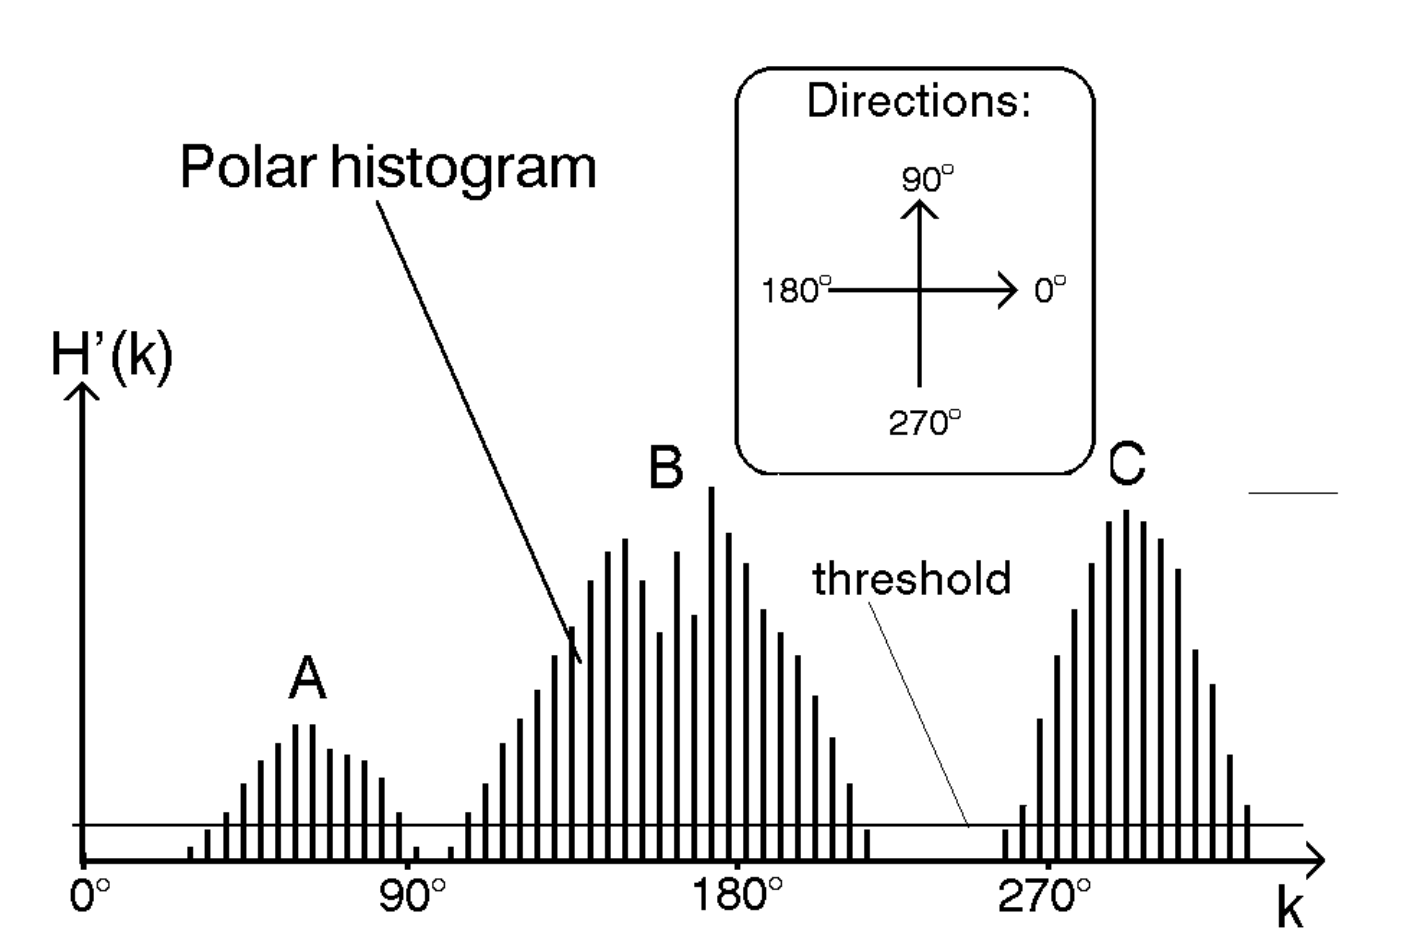
\includegraphics[width=0.55\textwidth]{img/polar_histogram}
    \caption{Histograma polar de magnitudes, com um valor empírico de
      limiar(threshold) de definição de um vale. Fonte: \cite{c1}}
    \label{fig:polar_hist}
\end{figure}

\begin{lstlisting}[frame=single, label=cod:vales, style=customc, caption={Algoritmo de Verificação de Vales}]
int VFH::getVales(float* vales, sensor_msgs::LaserScan msg){
    
    int sec_counter = 0; //Contador de setores por vale
    int num_vales = 0; //Contador de setores por vale
    
    //A cada setor de -angulo_abertura a angulo_abertura, verifica os possiveis vales
    for (float alpha = (-1)*angulo_abertura; alpha < angulo_abertura; alpha += angulo_setor){
        
        float c = 1; //Probabilidade de haver um obstaculo no setor
        float dist_setor = getDistanceAverage(alpha, msg, 5); //Range do setor atual
        float m = pow(c,2) * (a - b * dist_setor); //Calcula magnitude
        
        //Verifica possiveis vales
        //Se o valor atual for maior que o limite (ou percorreu todas as amostras)
        if (m > limite || alpha+angulo_setor >= angulo_abertura){
            if (sec_counter >= s_max) //Se o vale tiver o numero minimo de setores
                vales[num_vales++] = alpha - (sec_counter * angulo_setor)/2; //Calcula angulo central resultante do vale
            
            //Reseta o contador
            sec_counter = 0;
        }
        else sec_counter++;
    }
    return num_vales;
}
\end{lstlisting}


Se nenhum vale for encontrado, o robô para e gira em torno do próprio
eixo. Caso sejam encontrados um ou mais vales, é escolhido o vale cuja
direção seja a mais próxima da direção em que o robô é ordenado a
seguir. Durante este processo a velocidade do robô é limitada, de modo
que ele não venha a colidir com o obstáculo do qual ele está
desviando.

\begin{lstlisting}[frame=single, label=cod:vales, style=customc, caption={Escolha da direção e velocidade}]
(...)
  //Se nao encontrou nenhum vale
    if (num_vales == 0){
        twist_teleop.linear.x = 0; //Fica parado
        twist_teleop.angular.z = -1; //E girando em torno do proprio eixo
    }
    
    //Encontrou vale(s)
    else {
        //Escolhe o angulo referente ao vale mais proximo
        twist_teleop.angular.z = nearestAngle(twist_teleop.angular.z, vales, num_vales);
        
        //Controle da velocidade
        float c = 1; //Probabilidade de haver um obstaculo no setor
        float dist_vale = getDistanceAverage(twist_teleop.angular.z, msg, 5); //Range do vale escolhido
        float m = pow(c,2) * (a - b*dist_vale); //Calcula magnitude
        
        twist_teleop.linear.x *= (1 - fmin(m, hm)/hm); //Controla a velocidade do robo pela magnitude do vale
        
        //Controla a velocidade pela diferenca angular
        twist_teleop.linear.x = twist_teleop.linear.x *
            (1 - fabs(1.5 * twist_teleop.angular.z)/angulo_abertura) + MIN_SPEED;
    }
    
    //Retorna o vetor resultante
    return twist_teleop;

\end{lstlisting}

\subsection{Leituras do Laser}

Para as amostras do sensor, foi utilizado um filtro baseado na média
temporal dos valores fornecidos, visando a eliminação de eventuais
ruídos na leitura (Código \ref{cod:laser_callback}).

\begin{lstlisting}[frame=single, label=cod:laser_callback, style=customc, caption={Filtro de amostras do laser}]
void laserCallback(sensor_msgs::LaserScan scan)
{
    
    laserScanBuffer.push_back(scan);
    if(laserScanBuffer.size() > 40)
    {
        // Erases oldest element
        laserScanBuffer.erase(laserScanBuffer.begin());
    }
    
    scan_mem = scan;
    //ROS_INFO("%f\t%f", scan.range_min, scan.range_max);
    for(auto laserScan : laserScanBuffer)
    {
        for(auto range = scan.range_min ; range < scan.range_max ; range++)
        {
            scan_mem.ranges[range] += laserScan.ranges[range];
        }
    }
    
    for(auto range = scan.range_min ; range < scan.range_max ; range++)
    {
        scan_mem.ranges[range] /= laserScanBuffer.size();
    }
    
    //Informa inicializacao da scan_mem
    scan_mem_active = 1;
    
}
\end{lstlisting}



\section{Conclusão}
A partir desse estudo, foi possível implementar, simular e colocar 
em prática a movimentação do robô sem colidir com obstáculos. O VFH
se mostrou uma alternativa válida para esse desafio; com apenas o 
comando de direção e a navegação sensorial, o robô mostrou uma autonomia
para explorar um espaço bidimensional sem maiores problemas. Mesmo quando
submetido ao surgimento abrupto de obstáculos em sua frente, este mostrou-se
capaz de tomar decisões rápidas e eficazes, de forma que fosse evitada a
colisão e também o que tange o replanejamento de trajetória. Parte disso deve-se à
boa performance do algoritmo, capaz de realizar cálculos em tempo real, mesmo
com a limitação de processamento do embarcado; é também razoável levar em
consideração a taxa de atualização do sensor, que providencia uma ampla 
amostra de dados, possibilitando trabalhar sempre com o ambiente mais atual.


\section{Referências}
\renewcommand{\section}[2]{}
\begin{thebibliography}{depth}

\bibitem{c1} THE VECTOR FIELD HISTOGRAM - FAST OBSTACLE AVOIDANCE FOR MOBILE ROBOTS, J. Borenstein, Member, IEEE and Y. Koren, Senior Member, IEEE The University of Michigan, Ann Arbor Advanced Technology Laboratories  http://www-personal.umich.edu/~johannb/Papers/paper16.pdf (Acessado em: 01/dez/2016)

\bibitem{c2} SIMPLE, REAL-TIME OBSTACLE AVOIDANCE ALGORITHM FOR MOBILE ROBOTS, I. Susnea, V. Minzu, G. Vasiliu, Department of Control Engineering University “Dunarea de Jos”,  http://www.wseas.us/e-library/conferences/2009/tenerife/CIMMACS/CIMMACS-03.pdf (Acessado em: 02/dez/2016)

\bibitem{c3} ELASTIC BANDS: CONNETING, PATH PLANNING AND CONTROL, Khatib, O., Quinlan, S., Proceedings of IEEE International Conference on Robotics and Automation, Atlanta, GA, May 1993

\end{thebibliography}

\end{document}                   
